% !TeX program = xelatex
% Overleaf：编译器选择 XeLaTeX，主文档选择 main.tex。
% 空白模板；正文中的写作提示均为注释，不会出现在 PDF 中。
% 全国规范未统一字体、字号和行距；以下为可修改的模板默认值。
\documentclass[UTF8,a4paper,zihao=-4,fontset=fandol]{ctexart}
\usepackage[margin=2.7cm,footskip=1.2cm]{geometry}
\usepackage{amsmath,amssymb}
\usepackage{graphicx}
\usepackage{booktabs,tabularx}
\usepackage{tikz}
\usetikzlibrary{arrows.meta,positioning}
\usepackage{setspace}
\usepackage{fancyhdr}
\usepackage[hidelinks]{hyperref}

% Fandol 宋体/黑体随 TeX Live 提供，无须上传 Windows 字体。
\setstretch{1.3}
\setlength{\parindent}{2em}
\setlength{\parskip}{0pt}
\setlength{\textfloatsep}{10pt plus 2pt minus 2pt}
\setlength{\floatsep}{8pt plus 2pt minus 2pt}
\renewcommand{\topfraction}{0.90}
\renewcommand{\bottomfraction}{0.80}
\renewcommand{\textfraction}{0.08}
\renewcommand{\floatpagefraction}{0.75}
\raggedbottom
\ctexset{
  section = {
    name = {,、}, number = \chinese{section},
    format = \centering\heiti\zihao{4},
    aftername = {}, beforeskip = 1.2ex, afterskip = 0.8ex
  },
  subsection = {
    number = \arabic{section}.\arabic{subsection},
    format = \heiti\zihao{-4},
    beforeskip = 1ex, afterskip = 0.6ex
  },
  subsubsection = {
    number = \arabic{section}.\arabic{subsection}.\arabic{subsubsection},
    format = \heiti\zihao{-4}
  }
}
\setcounter{secnumdepth}{3}

% 页码从摘要开始连续编号，无页眉、横线和身份字段。
\pagestyle{fancy}
\fancyhf{}
\fancyfoot[C]{\small\thepage}
\renewcommand{\headrulewidth}{0pt}
\renewcommand{\footrulewidth}{0pt}
\hypersetup{pdfauthor={},pdftitle={},pdfsubject={},pdfkeywords={}}

% 2026 年 A 题论文标题，可在下面的花括号中修改。
\newcommand{\papertitle}{药材烘干过程的热质传递与干燥时长建模}
% 空白段落用于保持空模板的分页；填入正文后可删除对应命令。
\newcommand{\blankcontent}{\par\noindent\strut\par}

\begin{document}
\pagenumbering{arabic}

% ==================== 摘要专用页 ====================
% 标题、摘要和关键词合计原则上不得超过一页；不需要英文摘要。
% 不使用 titlepage 环境，避免摘要页码被隐藏或重新计数。
\begin{center}
  {\heiti\zihao{3}\strut\papertitle\par}
  \vspace{1em}
  {\heiti\zihao{4}摘要\par}
\end{center}
% 在此填写摘要。
\hspace*{2em}药材烘干过程中温度升高、水分外迁与几何收缩同时发生，直接决定产品能否达到安全含水率。本文以圆柱形药材为对象，建立从预热到恒温干燥、再到径向收缩的统一热质传递模型。

针对问题一，将药材简化为一维轴对称圆柱，分别建立径向热传导方程和非线性水分扩散方程，以附件1的环境温度和环境水分指标作为Robin边界，采用表面加密有限体积、后向Euler格式及Picard迭代求解。1800~s时中心与表面温度分别为$33.5754^\circ\mathrm C$、$36.7856^\circ\mathrm C$，干基含水率分别为2.5500、1.5102~kg/kg。针对问题二，引入随含水率、温度变化的密度、比热、导热系数和扩散系数，形成温度场与浓度场双向参数耦合模型；3~h时中心温度为$49.8495^\circ\mathrm C$，中心含水率为1.7662~kg/kg。针对问题三，以全部网格单元及中心、表面重构值的最大值为严格判据，通过保存未达标状态、重新积分和区间缩小定位首次达标时刻，得到总烘干时间约57.47~h。快速口径对照表明，若改用平均含水率判据，终点将提前约21.4~h。针对问题四，利用附件2全部145个半径数据作保形分段三次Hermite插值，通过材料坐标变换将移动区域映射到固定参考域，得到考虑收缩后的达标时间约51.09~h；在附录4同物性下，固定半径对照约为129.84~h，收缩使模型预测时长缩短60.7\%。

网格和步长加密后，问题三、四终点变化均小于0.1~s；四问最大水量收支残差不超过$2.54\times10^{-12}$~kg/kg。单因素筛选表明，环境温度和水分扩散系数是达标时间的主要驱动因素。模型能够在物理机制清晰、数值守恒的前提下预测药材内部温湿演化，并为烘干工艺参数选择提供量化依据。
\par\vspace{0.5em}
\noindent\hspace*{2em}\textbf{关键词：}药材烘干；热质耦合；有限体积法；移动边界；事件定位
% 在此填写关键词。
\par
\clearpage

% ==================== 正文，不设置目录 ====================
% 可选：引言；取消下一组注释即可启用，不参与正文编号。
% \section*{引言}
% \blankcontent

\section{问题重述}
\label{sec:restatement}
\subsection{问题背景}
烘干是药材加工和贮藏中的关键环节。外部热空气首先加热表层，随后热量向内部传导；与此同时，内部水分在浓度梯度驱动下向表面迁移并散入环境。温度、含水率以及材料尺寸在时间和空间上的非均匀性，使仅用平均含水率或单一经验干燥曲线难以准确判断最慢干燥位置。经典干燥研究将过程分为预热、近恒温及降速阶段\cite{lewis1921}，而分布参数模型可通过同时求解热传导与扩散方程描述内部场量\cite{pumpkin2017}。

题目给出圆柱形药材的初始尺寸、温度与干基含水率，附件1给出0--4~h环境驱动数据，附件2给出0--72~h半径变化数据，并在各问附录中给出物性参数或经验公式，需据此建立可计算、可检验且能按指定位置输出结果的数学模型。
% 可选：现实应用图。将文末图片骨架复制到此处，并填入实际图片路径。
\subsection{基本问题}
本文依次完成四项任务：第一，建立前1800~s预热阶段的温度和水分浓度模型；第二，引入变物性经验公式，描述0--3~h完整烘干过程中的热质耦合；第三，以全域干基含水率严格低于0.15~kg/kg为标准，确定首次达标时间；第四，考虑半径随时间缩小，将固定区域模型推广为移动边界模型，并比较收缩与固定半径方案的差异。
% 可选：总体思路框架；不启用时无需保留空图。
% \subsection{总体思路框架}
% \blankcontent

\section{模型假设}
\label{sec:assumptions}
\begin{enumerate}
  \item 药材初始为半径$R_0=0.02$~m、长度$L=0.25$~m的圆柱体，轴向长度远大于半径；忽略端部效应，只研究代表性截面的径向传递。
  \item 截面内材料宏观均匀且轴对称，温度$T(r,t)$和干基含水率$C(r,t)$连续变化；中心不存在净热流和水分通量。
  \item 环境温度和环境水分指标是表面对流边界的驱动量。题给环境水分指标作为药材侧的等效边界驱动，不把空气含湿量与固体干基含水率的质量基准直接等同。
  \item 问题一采用附录2常物性；问题二、三采用附录3变物性；问题四采用附录4变物性。经验公式在题给变量范围及数值延拓范围内有效。
  \item 表面对流换热系数$h=25$~W/(m$^2\cdot$K)、传质系数$h_m=8\times10^{-7}$~m/s在计算中保持不变。模型不显式计入蒸发潜热、辐射和化学反应热，因此温度结果只在题给有效物性和边界参数的口径下解释。
  \item 问题三、四超过附件1的4~h后，环境维持$50^\circ\mathrm C$和0.0500~kg/kg；问题四超过半径观测范围时维持末值。实际计算终点未超过72~h半径观测范围。
  \item 问题四只发生径向同比收缩，轴向长度不变；材料质点的干物质质量守恒，干基含水率随材料坐标演化。
\end{enumerate}

\section{符号说明}
\label{sec:notation}
\begin{center}
\renewcommand{\arraystretch}{1.3}
\small
\begin{tabularx}{0.95\textwidth}{c >{\raggedright\arraybackslash}X c}
\toprule
符号 & 含义 & 单位 \\
\midrule
$r,x,\xi$ & 物理径向坐标、参考径向坐标和无量纲材料坐标 & m，m，1\\
$R_0,R(t),s(t)$ & 初始半径、时变半径及缩放比$R(t)/R_0$ & m，m，1\\
$t$ & 从题设初态起算的时间 & s\\
$T,T_\infty,T_s$ & 药材温度、环境温度和表面温度 & K（结果以$^\circ$C报告）\\
$C,C_\infty^{\rm eff},C_s$ & 干基含水率、环境水分指标及表面含水率 & kg/kg\\
$\rho,c_p,k,D$ & 密度、比热容、导热系数和有效扩散系数 & kg/m$^3$，J/(kg$\cdot$K)，W/(m$\cdot$K)，m$^2$/s\\
$h,h_m$ & 表面对流换热系数和传质系数 & W/(m$^2\cdot$K)，m/s\\
$V_i,A_{i+1/2}$ & 圆柱壳体积权重和界面面积权重 & m$^2$，m\\
$G_{i+1/2},G_s$ & 内部界面及表面等效传递系数 & 随场量而定\\
$M_3(t),M_4(t),g(t)$ & 问题三、四的全域含水率最大值及阈值事件函数 & kg/kg\\
$\rho_d,L(t),B(t)$ & 干物质体积密度、累计失水及水量收支残差 & kg/m$^3$，kg/kg，kg/kg\\
$S_p,\tau$ & 归一化灵敏度和时间步长尺度 & 1，s\\
$N,\Delta t,\varepsilon_t$ & 控制体数、实际时间步长和事件定位容差 & 1，s，s\\
\bottomrule
\end{tabularx}
\end{center}

\begin{figure}[htbp]
  \centering
  \begin{tikzpicture}[
    node distance=5mm,
    box/.style={draw=black!65,rounded corners=2pt,fill=blue!5,minimum height=15mm,
                text width=3.0cm,align=center,font=\small},
    arrow/.style={-{Latex[length=2.2mm]},thick,draw=black!65}
  ]
    \node[box] (q1) {问题一\\常热物性传热\\非线性水分扩散};
    \node[box,right=of q1] (q2) {问题二\\变物性耦合\\重新从初态计算};
    \node[box,right=of q2] (q3) {问题三\\全域达标判定\\终止事件定位};
    \node[box,right=of q3] (q4) {问题四\\材料坐标变换\\给定半径收缩};
    \draw[arrow] (q1) -- (q2); \draw[arrow] (q2) -- (q3); \draw[arrow] (q3) -- (q4);
    \node[draw=black!50,fill=gray!7,below=7mm of q2,minimum height=9mm,
          text width=9.0cm,align=center,font=\small] (method)
          {统一数值框架：圆柱壳有限体积 $+$ 后向Euler $+$ Picard迭代\\
           统一输出：径向场、全域判据、水量守恒与网格/步长加密检验};
    \draw[arrow] (method.west) -| (q1.south);
    \draw[arrow] (method.east) -| (q4.south);
  \end{tikzpicture}
  \caption{四个问题的递进关系与统一求解框架}
  \label{fig:workflow}
\end{figure}

\section{问题一的建模与求解}
\label{sec:problem1}
\subsection{问题分析}
预热阶段的主要矛盾是表面受热、失水快，而内部对边界变化存在明显滞后。圆柱轴对称条件下，热量和水分均沿径向传递，可分别用Fourier热传导和Fick扩散描述\cite{crank1975}。附录2中热物性为常数，扩散系数只依赖含水率，因此温度方程不受水分场反馈，水分方程仍是非线性扩散方程。
% 可选：思维框架图；使用实际图片时再启用图片骨架。
\subsection{数据预处理}
附件1共241个观测点，时间为0--14400~s，间隔60~s。温度范围为$28.000$--$50.246^\circ\mathrm C$，环境水分指标范围为0.01963--0.05025~kg/kg。本文保留全部观测点，不平滑、不拟合，在相邻节点间采用分段线性插值
\begin{equation}
 y_\infty(t)=y_j+\frac{y_{j+1}-y_j}{t_{j+1}-t_j}(t-t_j),
 \quad t_j\le t\le t_{j+1},
 \label{eq:pwl}
\end{equation}
其中$y$分别代表$T_\infty$和$C_\infty^{\rm eff}$。摄氏温度在进入物性公式前转换为开尔文。结果先以未舍入浮点数保存，再按题目要求输出到\texttt{result1.xlsx}。
% 各问题共用的预处理可集中在此，后续问题引用本小节而不重复叙述。
\label{sec:preprocessing}
\subsection{可视化分析}
图~\ref{fig:environment}显示环境温度总体上升并逐渐接近$50^\circ\mathrm C$，环境水分指标也随时间上升。两者均具有局部波动，因此数值积分必须对齐数据节点，避免大时间步跨越边界折点。
\begin{figure}[htbp]
  \centering
  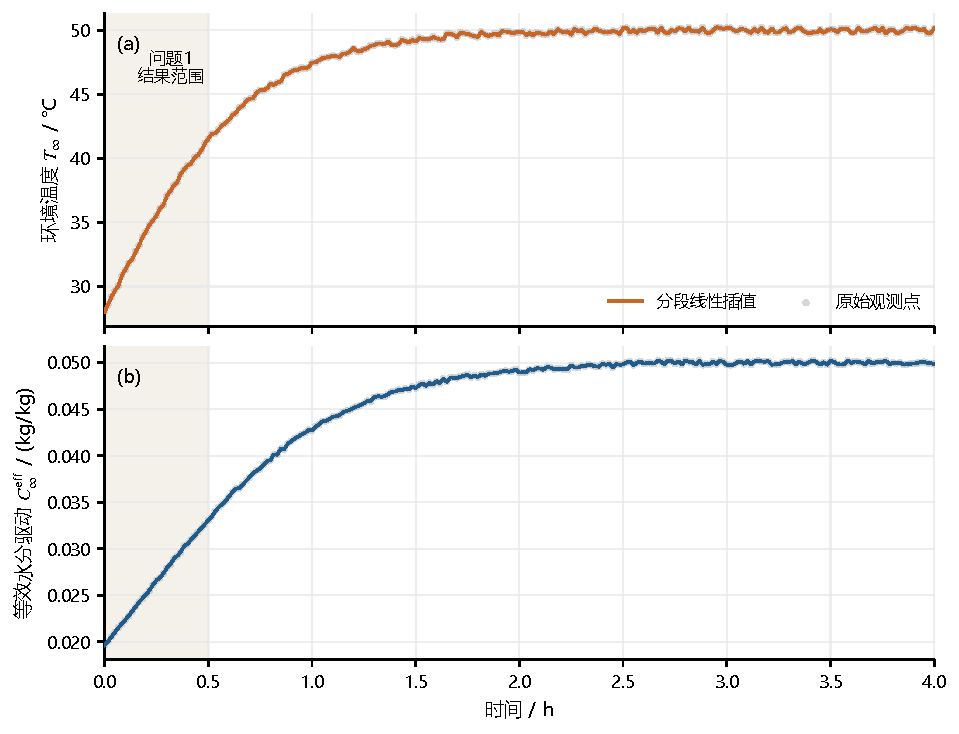
\includegraphics[width=0.86\linewidth]{q1/figures/fig1_environment.pdf}
  \caption{附件1环境温度与环境水分指标的时间变化}
  \label{fig:environment}
\end{figure}
\subsection{模型建立}
\subsubsection{控制方程}
在$0<r<R_0$上建立
\begin{align}
 \rho c_p\frac{\partial T}{\partial t}
 &=\frac1r\frac{\partial}{\partial r}\left(rk\frac{\partial T}{\partial r}\right),\label{eq:q1heat}\\
 \frac{\partial C}{\partial t}
 &=\frac1r\frac{\partial}{\partial r}\left(rD(C)\frac{\partial C}{\partial r}\right).\label{eq:q1mass}
\end{align}
式~\eqref{eq:q1heat}表示单位体积热储存率等于径向净导热通量，式~\eqref{eq:q1mass}表示干基含水率的变化由内部有效扩散通量决定。附录2给出
\begin{equation}
 \rho=820,\quad c_p=2600,\quad k=0.36,\quad
 D(C)=7.0\times10^{-9}\exp\!\left(-\frac{0.89}{C}\right).
 \label{eq:q1prop}
\end{equation}

\subsubsection{初始条件与边界条件}
\begin{align}
 T(r,0)&=301.15~{\rm K},& C(r,0)&=2.55,\label{eq:initial}\\
 \frac{\partial T}{\partial r}(0,t)&=0,&
 \frac{\partial C}{\partial r}(0,t)&=0,\label{eq:centerbc}\\
 -k\frac{\partial T}{\partial r}(R_0,t)&=h(T_s-T_\infty),&
 -D\frac{\partial C}{\partial r}(R_0,t)&=h_m(C_s-C_\infty^{\rm eff}).\label{eq:robin}
\end{align}
中心Neumann条件体现轴对称性；表面Robin条件把材料内部半单元传递阻力与外部对流阻力串联。计算域和边界含义见图~\ref{fig:radialmodel}。
\begin{figure}[htbp]
  \centering
  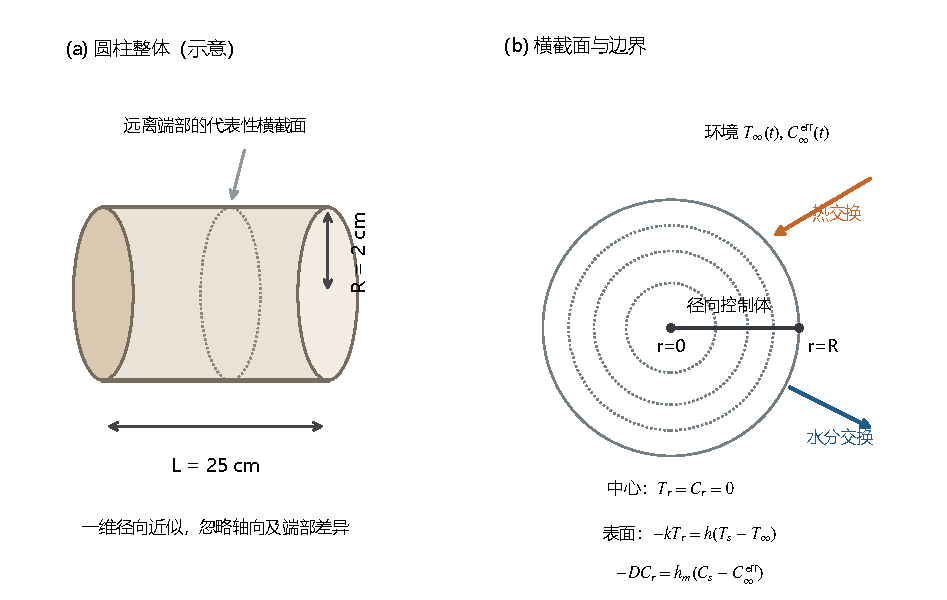
\includegraphics[width=0.74\linewidth]{q1/figures/fig2_radial_model.pdf}
  \caption{固定半径圆柱的径向热质传递模型}
  \label{fig:radialmodel}
\end{figure}
% 按实际模型细分三级标题；公式骨架见文末注释。
\subsection{算法与求解}
采用守恒型圆柱壳有限体积法\cite{patankar1980}。省略各壳共有因子$2\pi L$，第$i$个控制体及界面权重为
\begin{equation}
 V_i=\frac{r_{i+1/2}^2-r_{i-1/2}^2}{2},\quad
 A_{i+1/2}=r_{i+1/2},\quad
 \bar r_i=\frac23\frac{r_{i+1/2}^3-r_{i-1/2}^3}
 {r_{i+1/2}^2-r_{i-1/2}^2}.
\end{equation}
为解析初始表面陡梯度，令$x_j=j/N$，使用
\begin{equation}
 r_{j+1/2}=R_0\frac{10x_j-x_j^{10}}9,\qquad j=0,\ldots,N
\end{equation}
构造表面加密网格。对任一通量系数$b$，内部和表面等效传递系数分别为
\begin{align}
 G_{i+1/2}&=\frac{A_{i+1/2}}
 {({r_{i+1/2}-\bar r_i})/{b_i}+({\bar r_{i+1}-r_{i+1/2}})/{b_{i+1}}},\\
 G_s&=\frac{R_0}{(R_0-\bar r_N)/b_N+1/\beta},
\end{align}
热量取$(b,\beta)=(k,h)$，水分取$(D,h_m)$。后向Euler离散为
\begin{equation}
 m_iV_i\frac{u_i^{n+1}-u_i^n}{\Delta t}
 =G_{i-1/2}(u_{i-1}^{n+1}-u_i^{n+1})
 +G_{i+1/2}(u_{i+1}^{n+1}-u_i^{n+1}),
 \label{eq:be}
\end{equation}
表面右通量换为$G_s(u_\infty^{n+1}-u_N^{n+1})$。热量方程$m_i=\rho c_p$，水分方程$m_i=1$。冻结物性后形成三对角方程；水分场通过Picard迭代更新$D(C)$，同时检查状态增量与离散残差。正式计算取$N=960$，时间尺度$\tau=1/768$~s，目标步长为$\tau(1+t/600)^2$且不超过$4\tau$，所有整数秒和环境节点精确对齐。后向Euler对线性扩散无条件稳定，非线性部分仍由迭代收敛和步长回退控制。
% 可选：算法流程图；插入已绘制的流程图即可。
\subsection{结果分析}
图~\ref{fig:q1profiles}给出七个时刻的径向剖面。温度由表面向中心传播，水分则由表面首先降低，中心在1800~s内几乎保持初值，说明预热和失水存在显著空间滞后。
\begin{figure}[htbp]
  \centering
  
\includegraphics[width=0.92\linewidth]{q1/figures/fig3_q1_profiles.pdf}
  \caption{问题一温度与干基含水率的径向演化}
  \label{fig:q1profiles}
\end{figure}
\begin{table}[htbp]
\centering\small
\caption{问题一代表时刻温度（$^\circ$C）}\label{tab:q1t}
\begin{tabular}{crrrrr}
\toprule
$t$/s&\multicolumn{5}{c}{径向位置 $r$/cm}\\\cmidrule(lr){2-6}
&0&0.5&1.0&1.5&2.0\\\midrule
100&28.0001&28.0003&28.0040&28.0327&28.1801\\
300&28.0408&28.0635&28.1514&28.3681&28.8489\\
600&28.4533&28.5360&28.8039&29.3159&30.1652\\
900&29.3243&29.4583&29.8755&30.6161&31.7304\\
1200&30.5427&30.7098&31.2224&32.1126&33.4276\\
1500&31.9957&32.1867&32.7660&33.7463&35.1203\\
1800&33.5754&33.7720&34.3642&35.3621&36.7856\\\bottomrule
\end{tabular}
\end{table}
\begin{table}[htbp]
\centering\small
\caption{问题一代表时刻干基含水率（kg/kg）}\label{tab:q1c}
\begin{tabular}{crrrrr}
\toprule
$t$/s&\multicolumn{5}{c}{径向位置 $r$/cm}\\\cmidrule(lr){2-6}
&0&0.5&1.0&1.5&2.0\\\midrule
100&2.5500&2.5500&2.5500&2.5500&2.2470\\
300&2.5500&2.5500&2.5500&2.5492&2.0508\\
600&2.5500&2.5500&2.5500&2.5353&1.8770\\
900&2.5500&2.5500&2.5497&2.5045&1.7547\\
1200&2.5500&2.5500&2.5482&2.4646&1.6586\\
1500&2.5500&2.5499&2.5445&2.4206&1.5787\\
1800&2.5500&2.5497&2.5383&2.3755&1.5102\\\bottomrule
\end{tabular}
\end{table}
1800~s时表面比中心高$3.2102^\circ\mathrm C$，中心比表面高1.0398~kg/kg；干物质质量加权平均含水率约为2.2936~kg/kg，累计失水约为0.2564~kg/kg。结果表明该阶段尚未达到内部热湿平衡，表面测量不能代表全域最湿位置。

\section{问题二的建模与求解}
\label{sec:problem2}
\subsection{问题分析}
完整烘干过程中，含水率下降会改变密度、比热和导热系数，温度又通过Arrhenius项影响扩散系数，因此需将问题一的弱耦合模型改为变物性热质耦合模型。问题二从题设均匀初态独立计算0--3~h，全部时段统一使用附录3参数，不与问题一1800~s结果拼接。
% 可选：思维框架图；使用实际图片时再启用图片骨架。
\subsection{数据预处理}
环境驱动沿用第~\ref{sec:preprocessing}~节的分段线性插值。为避免单位错误，环境温度先加273.15，所有扩散系数公式中的$T$均使用K。输出每秒、21个固定径向位置的未舍入结果，最后生成\texttt{result2.xlsx}；表格展示时保留四位小数。
% 共用处理可引用第~\ref{sec:preprocessing}~节，并仅补充本问题的特有处理。
\subsection{可视化分析}
图~\ref{fig:q2evolution}同时展示温度场、含水率场和典型位置曲线。约2~h后温度场已接近环境温度，径向温差显著缩小；水分场仍保留较大梯度，说明恒温不等于水分平衡，后续时长主要由内部扩散控制。
\begin{figure}[htbp]
  \centering
  
\includegraphics[width=0.85\textwidth]{q2/figures/fig4_q2_evolution.pdf}
  \caption{问题二0--3 h温度场与含水率场演化}
  \label{fig:q2evolution}
\end{figure}
\subsection{模型建立}
控制方程和初边值形式仍为式~\eqref{eq:q1heat}--\eqref{eq:robin}，但物性更新为
\begin{align}
 \rho(C)&=650+128C,\qquad
 c_p(C)=1450+2736\frac{C}{C+1},\\
 k(C)&=0.21+0.38\frac{C}{C+1},\\
 D(C,T)&=2.4\times10^{-3}\exp\!\left(-\frac{0.45}{C}\right)
 \exp\!\left(-\frac{3850}{T}\right).\label{eq:q2prop}
\end{align}
耦合路径为
\[
 C\longrightarrow \{\rho,c_p,k\}\longrightarrow T,\qquad
 (T,C)\longrightarrow D\longrightarrow C.
\]
即含水率通过热储存和导热能力改变温度场，温度和含水率共同改变扩散能力；这种基于机理的耦合在生物材料对流干燥模型中具有明确物理基础\cite{biomass2020}。模型未显式加入潜热项，因此所得温度场是题给有效参数口径下的预测。
% 按实际模型细分三级标题；公式骨架见文末注释。
\subsection{算法与求解}
空间离散仍采用问题一的圆柱壳有限体积格式。每个时间步内依次执行：由当前猜测$(T^{(q)},C^{(q)})$计算$\rho c_p$与$k$；求解温度三对角系统得到$T^{(q+1)}$；用$(T^{(q+1)},C^{(q)})$更新$D$并求解水分系统；检查两个场的归一化增量；用候选新状态重算物性并检查式~\eqref{eq:be}残差。绝对和相对容差分别为$10^{-10}$、$10^{-11}$，若迭代恶化则阻尼或回退时间步，不对含水率作截断。正式计算取$N=960$、$\tau=1/768$~s，累计2,194,220个接受步。
% 可选：算法流程图；插入已绘制的流程图即可。
\subsection{结果分析}
\begin{table}[htbp]
\centering\small
\caption{问题二代表时刻温度（$^\circ$C）}\label{tab:q2t}
\begin{tabular}{crrrrr}
\toprule
$t$/h&\multicolumn{5}{c}{径向位置 $r$/cm}\\\cmidrule(lr){2-6}
&0&0.5&1.0&1.5&2.0\\\midrule
0.5&32.1893&32.3821&32.9659&33.9608&35.4130\\
1.0&40.3816&40.5536&41.0605&41.8782&42.9976\\
1.5&45.8468&45.9348&46.1930&46.6051&47.1400\\
2.0&48.4502&48.4881&48.5984&48.7735&49.0033\\
2.5&49.4670&49.4792&49.5136&49.5653&49.6609\\
3.0&49.8495&49.8553&49.8746&49.9101&49.9664\\\bottomrule
\end{tabular}
\end{table}
\begin{table}[htbp]
\centering\small
\caption{问题二代表时刻干基含水率（kg/kg）}\label{tab:q2c}
\begin{tabular}{crrrrr}
\toprule
$t$/h&\multicolumn{5}{c}{径向位置 $r$/cm}\\\cmidrule(lr){2-6}
&0&0.5&1.0&1.5&2.0\\\midrule
0.5&2.5499&2.5489&2.5256&2.3257&1.6486\\
1.0&2.5257&2.4948&2.3578&2.0230&1.4711\\
1.5&2.3861&2.3256&2.1344&1.8020&1.3476\\
2.0&2.1709&2.1084&1.9236&1.6259&1.2311\\
2.5&1.9566&1.9006&1.7360&1.4720&1.1166\\
3.0&1.7662&1.7165&1.5702&1.3333&1.0081\\\bottomrule
\end{tabular}
\end{table}
3~h时中心与表面温差仅$0.1169^\circ\mathrm C$，但含水率差仍为0.7581~kg/kg；平均含水率约为1.3825~kg/kg，累计失水约为1.1675~kg/kg。这验证了“预热阶段受热响应显著、恒温阶段扩散控制占主导”的阶段差异，也说明问题三必须以内部最大含水率而非平均值判定终点。

\section{问题三的建模与求解}
\label{sec:problem3}
\subsection{问题分析}
第三问不是在离散输出表中寻找第一个小于0.15的数，而是求连续时间数值模型中全域最大含水率首次严格越过阈值的时刻。由于中心是最慢干燥位置，四位小数显示为0.1500时仍可能位于阈值两侧，必须保留完整未舍入状态并实施事件定位。
% 可选：思维框架图；使用实际图片时再启用图片骨架。
\subsection{数据预处理}
读取问题二在$t_0=10800$~s时全部960个控制体的温度、含水率、网格与累计失水，不用21个展示点反插值。3--4~h继续使用附件1，4~h后按模型假设取$T_\infty=323.15$~K、$C_\infty^{\rm eff}=0.0500$~kg/kg。每60~s保存21个指定径向位置，非整分钟终点单独写入终点记录和\texttt{result3.xlsx}末行。
% 共用处理可引用第~\ref{sec:preprocessing}~节，并仅补充本问题的特有处理。
\subsection{可视化分析}
图~\ref{fig:q3endpoint}从题设初态起统一展示全域最大值、径向平均值及三个代表位置的含水率变化。中心始终是最慢干燥位置，因而控制最终烘干时间；平均值则会更早越过阈值。
\begin{figure}[htbp]
  \centering
  
\includegraphics[width=0.85\textwidth]{q3/figures/fig5_q3_drying_endpoint.pdf}
  \caption{问题三全域最大含水率的阈值交叉与含水率场}
  \label{fig:q3endpoint}
\end{figure}
\subsection{模型建立}
延续问题二的控制方程、附录3物性和固定半径。定义数值全域最大值
\begin{equation}
 M_h(t)=\max\{C_{\rm center}^{\rm rec},C_1,\ldots,C_N,C_{\rm surface}^{\rm bc}\},
 \qquad g_h(t)=M_h(t)-0.15.
 \label{eq:event}
\end{equation}
中心值用满足轴对称性的二次式$C(r)=\alpha+\beta r^2$，由首两个控制体体积平均值重构；表面值由与Robin通量一致的半单元公式重构。严格达标条件为未舍入的$g_h(t)<0$，这样既覆盖全部网格单元，也避免把末单元中心误当成真实表面。
% 按实际模型细分三级标题；公式骨架见文末注释。
\subsection{算法与求解}
普通续算阶段以$\Delta t_{\max}=0.03125$~s推进，每到60~s检查$M_h(t)$。当首次发现区间端点由未达标变为达标时，保存左端完整状态作为起始状态，对每个候选时刻重新积分，并用二分法约束上下界，直到
\begin{equation}
 g_h(t_-)\ge0,\quad g_h(t_+)<0,\quad t_+-t_-\le0.01~{\rm s}.
\end{equation}
该方法不在两个输出值之间直接线性插值，因而候选时刻始终对应实际数值积分状态；最终搜索区间宽度小于0.01~s，并取首次满足严格判据的一侧作为报告终点。该区间宽度仅反映事件搜索精度，不代表模型预测误差。
% 可选：算法流程图；插入已绘制的流程图即可。
\subsection{结果分析}
\begin{table}[htbp]
\centering\small
\caption{问题三各时刻干基含水率（kg/kg）}\label{tab:q3c}
\begin{tabular}{crrrrr}
\toprule
$t$/h&\multicolumn{5}{c}{径向位置 $r$/cm}\\\cmidrule(lr){2-6}
&0&0.5&1.0&1.5&2.0\\\midrule
6&1.0170&0.9881&0.9015&0.7550&0.5328\\
12&0.4561&0.4432&0.4031&0.3297&0.1642\\
18&0.2988&0.2915&0.2687&0.2253&0.0845\\
24&0.2378&0.2327&0.2167&0.1855&0.0665\\
30&0.2058&0.2018&0.1892&0.1641&0.0598\\
36&0.1859&0.1825&0.1718&0.1504&0.0566\\
42&0.1721&0.1691&0.1597&0.1407&0.0549\\
48&0.1618&0.1592&0.1507&0.1334&0.0537\\
54&0.1539&0.1514&0.1436&0.1277&0.0530\\
57.47&0.1500&0.1477&0.1402&0.1249&0.0527\\\bottomrule
\end{tabular}
\end{table}
得到从题设初态起算的总烘干时间
\[
t_{\rm finish}\approx206900~{\rm s}\approx57.47~{\rm h}.
\]
终点时未舍入的全域最大含水率刚好低于0.15~kg/kg，且位于$r=0$；表中0.1500为四位小数舍入值。末时刻平均含水率约0.1243~kg/kg，说明若以平均值作为判据会提前停机。前12~h表面快速失水，随后中心控制的降速阶段延续约45~h，提升后期效率应优先改善内部扩散或提高有效温度。

\section{问题四的建模与求解}
\label{sec:problem4}
\subsection{问题分析}
药材失水后半径缩小，一方面缩短水分和热量的传递路径，另一方面使物理计算域随时间移动。若直接在物理坐标上重构网格，需要处理网格速度与移动表面；本文利用同比收缩假设引入材料坐标，将移动边界问题转换为固定参考域上的变系数问题。
% 可选：思维框架图；使用实际图片时再启用图片骨架。
\subsection{数据预处理}
附件2含145个半径观测点，时间覆盖0--72~h，半径由2.000~cm降至1.198~cm。为保持单调性及观测平台，使用全部节点作保形分段三次Hermite插值（PCHIP）\cite{fritsch1980}，不另行拟合收缩机理。插值函数逐段检查未越过相邻观测值范围，92段相邻观测值相等的区间均被保留。结果输出时，对固定物理位置$r_j>R(t)$的单元留空，不以零或表面值填充。
% 共用处理可引用第~\ref{sec:preprocessing}~节，并仅补充本问题的特有处理。
\subsection{可视化分析}
图~\ref{fig:q4radius}左侧给出半径观测与插值曲线，右侧示意物理坐标$r$和固定材料坐标$\xi$的映射。终点附近半径已趋于1.2~cm，因此$r=1.5$~cm和2.0~cm已位于材料域外。
\begin{figure}[htbp]
  \centering
  
\includegraphics[width=0.95\linewidth]{q4/figures/fig6_q4_radius_mapping.pdf}
  \caption{附件2半径变化及移动域到参考域的坐标映射}
  \label{fig:q4radius}
\end{figure}
\subsection{模型建立}
令
\begin{equation}
 s(t)=\frac{R(t)}{R_0},\qquad x=\frac{r}{s(t)}\in[0,R_0],
 \qquad \xi=\frac{x}{R_0}=\frac{r}{R(t)}.
\end{equation}
设单位轴长内各材料壳的干物质质量守恒，则$\rho_d(t)R(t)^2=\rho_{d,0}R_0^2$，故$\rho_d\propto s^{-2}$。这里$\rho_d$只用于水量核算；热方程中的$a(C)=\rho(C)c_p(C)$是题给经验式构造的有效热储存系数，二者不强加额外密度关系。材料速度为$v_r=\dot s\,r/s$；由$r=s(t)x$可得
\begin{align*}
 \frac{\mathrm D}{\mathrm Dt}
 &=\left.\frac{\partial}{\partial t}\right|_r+v_r\frac{\partial}{\partial r}
 =\left.\frac{\partial}{\partial t}\right|_x,\\
 \frac{\partial}{\partial r}&=\frac1s\frac{\partial}{\partial x},
 \qquad r\,\mathrm dr=s^2x\,\mathrm dx,\\
 J_r&=-kT_r=-\frac{k}{s}T_x,
 \qquad J_{C,r}=-DC_r=-\frac{D}{s}C_x,\\
 \rho c_pT_t\big|_x&=\frac1x\partial_x\!\left(x\frac{k}{s^2}T_x\right),
 \qquad C_t\big|_x=\frac1x\partial_x\!\left(x\frac{D}{s^2}C_x\right).
\end{align*}
因此显式对流项不是被忽略，而是在随材料运动的坐标下自然并入材料导数；通量与面积元变换后得到下述参考域方程。附录4物性为
\begin{align}
 \rho&=760+90C,& c_p&=1850+2150\frac{C}{C+1},\\
 k&=0.12+0.20\frac{C}{C+1},&
 D&=4.2\times10^{-4}\exp\!\left(-\frac{0.30}{C}\right)
 \exp\!\left(-\frac{3850}{T}\right).
\end{align}
参考域控制方程为
\begin{align}
 \rho c_p\left.\frac{\partial T}{\partial t}\right|_x
 &=\frac1x\frac{\partial}{\partial x}
 \left(x\frac{k}{s^2}\frac{\partial T}{\partial x}\right),\label{eq:q4heat}\\
 \left.\frac{\partial C}{\partial t}\right|_x
 &=\frac1x\frac{\partial}{\partial x}
 \left(x\frac{D}{s^2}\frac{\partial C}{\partial x}\right).\label{eq:q4mass}
\end{align}
中心仍为零梯度，表面条件相应变为
\begin{align}
 -\frac{k}{s^2}T_x(R_0,t)&=\frac{h}{s}(T_s-T_\infty),\\
 -\frac{D}{s^2}C_x(R_0,t)&=\frac{h_m}{s}(C_s-C_\infty^{\rm eff}).
 \label{eq:q4bc}
\end{align}
因此收缩通过$1/s^2$增强内部等效传递，并通过$1/s$修正参考域表面交换；初始条件仍为式~\eqref{eq:initial}。这种把尺寸变化与热湿扩散共同纳入模型的处理与收缩食品干燥研究的基本思路一致\cite{rovedo1997}。
% 按实际模型细分三级标题；公式骨架见文末注释。
\subsection{算法与求解}
在固定$x$网格上复用有限体积、后向Euler和Picard算法，每个新时间层先由PCHIP计算$R(t_{n+1})$和$s(t_{n+1})$，再以$k/s^2$、$D/s^2$、$h/s$、$h_m/s$构造通量系数。全域事件判据为
\[
M_4(t)=\max_{0\le r\le R(t)}C(r,t)<0.15.
\]
正式计算取$N=1280$、普通和事件步长上限均为0.03125~s，事件定位容差0.01~s。水量核算仍按初始参考壳层的干物质质量权重进行：
\begin{equation}
 \bar C(t)=\frac{\sum_iV_iC_i(t)}{\sum_iV_i},\qquad
 B(t)=\bar C(t)+L(t)-2.55.
\end{equation}
% 可选：算法流程图；插入已绘制的流程图即可。
\subsection{结果分析}
\begin{table}[htbp]
\centering\scriptsize
\caption{考虑收缩时的干基含水率与半径}\label{tab:q4c}
\resizebox{\textwidth}{!}{
\begin{tabular}{crrrrrrr}
\toprule
$t$/h&\multicolumn{5}{c}{固定物理位置 $r$/cm}&表面&$R(t)$/cm\\\cmidrule(lr){2-6}
&0&0.5&1.0&1.5&2.0&&\\\midrule
6&1.7188&1.5370&1.0221&--&--&0.4205&1.3740\\
12&0.7374&0.6544&0.4082&--&--&0.1669&1.2480\\
18&0.4086&0.3686&0.2397&--&--&0.0892&1.2140\\
24&0.2851&0.2610&0.1790&--&--&0.0673&1.2040\\
30&0.2263&0.2094&0.1493&--&--&0.0595&1.2010\\
36&0.1928&0.1796&0.1316&--&--&0.0560&1.2000\\
42&0.1712&0.1604&0.1200&--&--&0.0541&1.2000\\
48&0.1561&0.1468&0.1116&--&--&0.0530&1.2000\\
51.09&0.1500&0.1413&0.1081&--&--&0.0526&1.2000\\\bottomrule
\end{tabular}}
\end{table}
严格终点约为
\[
t_{\rm finish}\approx183913~{\rm s}\approx51.09~{\rm h},
\]
终点时未舍入的全域最大含水率刚好低于0.15~kg/kg，位于中心，半径为1.2000~cm；事件搜索区间宽度小于0.01~s。图~\ref{fig:q4compare}比较附录4物性下收缩与固定半径模型，并给出收缩模型的中心、径向平均和表面含水率。附录4同物性固定半径对照的终点约为129.84~h，收缩使终点提前约78.75~h，即60.7\%。问题三与问题四同时改变了物性参数，故二者57.47~h与51.09~h之差不能全部归因于收缩；只有附录4同物性对照才能隔离几何效应。

\noindent\textbf{扩散时间尺度检验：}扩散主导过程的特征时间与半径平方成正比。若以末期半径1.198~cm和初始半径2.000~cm估算，则$(1.198/2)^2\approx0.359$；实际计算所得时间比为$51.09/129.84\approx0.393$。二者处于一致数量级，且实际收缩需要一定过程时间，说明移动边界模型的时间尺度具有合理性。
\begin{figure}[htbp]
  \centering
  
\includegraphics[width=0.85\textwidth]{q4/figures/fig7_q4_shrinking_comparison.pdf}
  \caption{问题四移动域含水率演化及同物性固定半径对照}
  \label{fig:q4compare}
\end{figure}

\section{模型的分析与检验}
\label{sec:validation}
\subsection{灵敏度分析}
采用问题三固定半径耦合模型作单因素局部筛选。为控制计算量，各方案统一取$N=120$，0--600~s、600--3600~s及之后的最大时间步分别为5、15、60~s；该筛选基准约为57.62~h，只用于比较相对变化，正式终点仍以$N=960$结果57.47~h为准。对$k,D,h,h_m$分别作$\pm10\%$扰动，对环境温度全时段作$\pm2^\circ\mathrm C$平移。对具有同量纲比例扰动的传递参数，定义中心差分归一化灵敏度
\begin{equation}
 S_p=\frac{t_+-t_-}{t_0}\bigg/\frac{p_+-p_-}{p_0},
 \label{eq:sensitivity}
\end{equation}
环境温度不作无量纲归一化，而直接报告单位温升引起的终点变化。
\begin{table}[htbp]
\centering\small
\caption{单因素扰动的达标时间与灵敏度}\label{tab:sensitivity}
\begin{tabular}{lrrr}
\toprule
参数&低水平达标时间/h&高水平达标时间/h&$S_p$\\\midrule
导热系数$k$&57.6233&57.6205&-0.0002\\
扩散系数$D$&63.3023&52.9970&-0.8942\\
环境温度$T_\infty$&61.5518&54.0291&--\\
换热系数$h$&57.6305&57.6146&-0.0014\\
传质系数$h_m$&58.3473&57.0539&-0.1122\\\bottomrule
\end{tabular}
\end{table}
环境温度每升高$1^\circ\mathrm C$，干燥终点约缩短1.9~h；扩散系数提高1\%，终点约缩短0.5~h。
完整的参数扰动图移至附录~\ref{app:numerical}，正文保留表~\ref{tab:sensitivity}所需的定量结果。
各传递参数的$S_p$均为负，温度的绝对变化也表明升温会缩短烘干时间。环境温度与扩散系数的影响最大，$h_m$次之；$k$与$h$影响很小，因为长时间阶段温度场已经接近恒温，终点主要由内部水分迁移决定。因此工艺优化应首先保证有效温度并改善内部扩散条件，同时注意过高温度可能引起有效成分损失，本模型未对品质约束建模。
% 仅在实际方法适用时，将小节细分或改名为：
% “基于鲁棒优化的灵敏度分析”“基于动态调参的灵敏度分析”。
\subsection{稳健性检验}
从空间、时间、非线性迭代、事件定位和守恒五个层面检验模型。
\subsubsection{终点判据和模型口径敏感性分析}
采用$N=120$快速设置对不同口径作同精度比较，并把分段最大时间步连续减半到基准设置的$1/8$；各方案末两级终点差均小于0.007~h。表~\ref{tab:criterion-robust}中的变化量均相对同精度的快速基准计算，正式结果另列，因而不会把离散差异混入口径影响。
\begin{table}[htbp]
\centering\small
\caption{问题三、四不同实现口径的终点比较}\label{tab:criterion-robust}
\begin{tabular}{lrrrr}
\toprule
方案 & 问题三/h & 变化/h & 问题四/h & 变化/h\\\midrule
本文正式计算 & 57.47 & -- & 51.09 & --\\
$N=120$同精度基准 & 57.48 & 0 & 51.09 & 0\\
4~h后保持附件末值 & 57.18 & $-0.30$ & 50.83 & $-0.27$\\
径向平均含水率判据 & 36.03 & $-21.45$ & 34.97 & $-16.12$\\
半径采用分段线性插值 & -- & -- & 51.10 & $+0.004$\\\bottomrule
\end{tabular}
\end{table}
环境延拓会带来约十几分钟差异；平均含水率不能保证中心达标，会过早终止；在相同材料坐标模型内，PCHIP与线性半径插值的影响不足一分钟。由此可见，第三、四问的小时级偏差主要来自达标判据和移动边界建模口径，而不是事件搜索精度。

\subsubsection{数值收敛与守恒检验}
问题一、二空间加密的最大含水率差均小于$10^{-5}$~kg/kg；问题三、四的空间、时间及事件步长加密后，终点变化均小于0.1~s。将Picard容差收紧100倍，问题四含水率最大差为$4.09\times10^{-13}$~kg/kg。四问最大水量收支残差不超过$2.54\times10^{-12}$~kg/kg。详细加密表和收敛图移至附录~\ref{app:numerical}，避免数值验证挤占模型论证篇幅。

在物理合理性方面，模型均预测“表面先升温、先失水，中心后响应且最终控制终点”，与对流干燥的一般规律一致。将4~h后环境改为保持附件末值，问题三匹配精度算例的终点变化约为$-18.2$~min（$-0.53\%$），说明环境延拓假设的影响有限但不可忽略。由于题目未给内部温湿实测值，以上检验只能证明数值稳定性、守恒性和定性合理性，不能替代实验校准。

\section{模型的评价与推广}
\subsection{模型的优点}
\begin{enumerate}
  \item 控制方程、初边界条件和参数耦合均有明确物理意义，能输出任意时刻和位置的温度、含水率，而非只给经验终点。
  \item 有限体积离散保持局部与全局水量守恒，表面半单元阻力与Robin边界一致；中心、表面值均经物理约束重构。
  \item 问题三的严格事件判据覆盖全部网格单元并保留未舍入值，避免固定输出点和四位小数造成误判。
  \item 材料坐标把移动边界转换为固定域变系数问题，既保留附件2全部半径信息，又复用前三问的稳定求解框架。
\end{enumerate}
\subsection{模型的缺点}
模型参数主要来自题给经验公式，缺少针对具体药材批次的反演与实验验证；一维径向假设忽略端部、裂隙、纤维束和各向异性；未显式描述液态水蒸发潜热、气相输运、外部流场及品质成分衰减；问题四将半径数据视为外生输入，未建立含水率与收缩之间的反馈本构关系。
\subsection{模型改进方向}
可用内部温度、质量损失和半径实验数据同时反演$D,h_m$及收缩本构参数，并给出置信区间；进一步建立含潜热、液气两相输运和黏弹性收缩的二维轴对称或三维模型；在大量批次数据可用时，可用物理约束机器学习预测随品种、温度和含水率变化的有效参数，但应保持守恒方程作为结构约束，并用独立批次验证泛化误差。
\subsection{模型的推广}
只需替换几何、物性经验式和环境边界，本框架可用于根茎类药材、果蔬、木材和生物质颗粒的对流干燥；将阈值函数改为温度上限、活性成分保留率或能耗函数后，可进一步用于多目标工艺优化、分阶段温度控制和在线剩余烘干时间预测。

% ==================== 声明与参考文献 ====================
\section*{AI工具使用声明}
本参赛队在论文整理和修订过程中使用了AI工具，主要用于LaTeX正文草拟、评审意见整理与落实、代码和结果文件的结构化核对、图表版式检查及编译错误排查。控制方程、参数口径、程序计算和数值结论均以题目附件及支撑材料中的实际运行结果为准，并通过独立复现、加密计算和水量守恒检查进行人工复核。详细使用情况随支撑材料另附说明。
% 按竞赛全过程的真实情况填写；以下两种规定表述二选一，不要同时启用。
% 未使用时：本参赛队在竞赛过程中未使用任何AI工具。
% 使用时：本参赛队在竞赛过程中使用了AI工具，主要用于〖简要用途〗，
% 详细使用情况见支撑材料。
% 使用时须在支撑材料中另附“AI工具使用详情.pdf”；详见 README.md。

\section*{参考文献}
\begingroup
\renewcommand{\refname}{}
\vspace{-2em}
\begin{thebibliography}{99}
  \bibitem{lewis1921} Lewis W K. The rate of drying of solid materials[J]. Journal of Industrial \& Engineering Chemistry, 1921, 13(5): 427--432. DOI: 10.1021/ie50137a021.
  \bibitem{pumpkin2017} Agrawal S G, Methekar R N. Mathematical model for heat and mass transfer during convective drying of pumpkin[J]. Food and Bioproducts Processing, 2017, 101: 68--73. DOI: 10.1016/j.fbp.2016.10.005.
  \bibitem{crank1975} Crank J. The Mathematics of Diffusion[M]. 2nd ed. Oxford: Clarendon Press, 1975.
  \bibitem{patankar1980} Patankar S V. Numerical Heat Transfer and Fluid Flow[M]. Washington: Hemisphere Publishing, 1980.
  \bibitem{biomass2020} Nagata G A, Costa T V, Perazzini M T B, Perazzini H. Coupled heat and mass transfer modelling in convective drying of biomass at particle-level: model validation with experimental data[J]. Renewable Energy, 2020, 149: 1290--1299. DOI: 10.1016/j.renene.2019.10.123.
  \bibitem{fritsch1980} Fritsch F N, Carlson R E. Monotone piecewise cubic interpolation[J]. SIAM Journal on Numerical Analysis, 1980, 17(2): 238--246. DOI: 10.1137/0717021.
  \bibitem{rovedo1997} Rovedo C O, Suárez C, Viollaz P E. Kinetics of forced convective air drying of potato and squash slabs[J]. Food Science and Technology International, 1997, 3(4): 251--261. DOI: 10.1177/108201329700300403.
\end{thebibliography}
\endgroup
% 有真实文献后，删除上面的“参考文献”标题和对应 \blankcontent，
% 改用以下环境（该环境自动生成标题），以免标题重复。
% \begin{thebibliography}{99}
%   \bibitem{ref:key} % 在此填写完整、真实的文献条目。
% \end{thebibliography}
% 在正文相应位置使用 \cite{ref:key}；不可只列文献而不标注引用。

% ==================== 附录，页码继续 ====================
\clearpage
\section*{附录}
\appendix
\ctexset{
  section = {name = {,}, number = \Alph{section}, aftername = \quad},
  subsection = {number = \Alph{section}.\arabic{subsection}},
  subsubsection = {
    number = \Alph{section}.\arabic{subsection}.\arabic{subsubsection}
  }
}
\section{支撑材料文件列表}
\label{app:files}
下表仅列随支撑材料提交的数据、程序与复核结果；正文排版直接使用的图文件不重复列入。
\begin{center}
\scriptsize
\renewcommand{\arraystretch}{1.08}
\begin{tabularx}{\textwidth}{l >{\raggedright\arraybackslash}X >{\raggedright\arraybackslash}X}
\toprule
文件名（含相对路径） & 内容说明 & 对应问题或用途 \\
\midrule
\nolinkurl{data/attachment1.xlsx}, \nolinkurl{data/attachment2.xlsx} & 环境温度、环境水分指标和半径变化原始数据 & 问题1--4输入\\
\nolinkurl{common/*.py}, \nolinkurl{q1/*.py}, \nolinkurl{q2/*.py} & 通用有限体积模块及前两问求解程序 & 问题1、2\\
\nolinkurl{q3/*.py}, \nolinkurl{q4/*.py} & 严格终点搜索、收缩域与半径插值程序 & 问题3、4\\
\nolinkurl{analysis/sensitivity_analysis.py} & 单因素灵敏度计算、CSV导出与绘图 & 模型分析\\
\nolinkurl{recalculation/build_v02_assets.py}, \nolinkurl{recalculation/convention_comparison.csv} & 口径对照补算、步长加密与修订图件生成 & 稳健性分析\\
\nolinkurl{submission_results/result1.xlsx}--\nolinkurl{result4.xlsx}, \nolinkurl{q1/tables}等 & 四份最终结果表及正文表格副本 & 问题1--4\\
\nolinkurl{validation/*.json}, \nolinkurl{validation/*.md} & 空间、时间、事件、守恒及独立复现记录 & 模型检验\\
\nolinkurl{paper_appendix_minimal/*.py} & 与工程代码解耦的完整最小复现程序 & 问题1--4复现\\
\bottomrule
\end{tabularx}
\end{center}
% 按实际支撑材料逐项填写；不要将模板 ZIP 作为支撑材料直接提交。
% 确实没有支撑材料时，删除空表并如实注明“本论文没有支撑材料”。

完整源程序代码及运行环境见支撑材料文件。

\section{详细数值验证}\label{app:numerical}
\begin{table}[htbp]
\centering\small
\caption{主要数值加密与守恒检验}
\begin{tabularx}{\textwidth}{l X r r}
\toprule
问题&检验方式&最大场差/(kg/kg)&终点差/s\\\midrule
1&$N=960\to1280$空间加密&$4.070\times10^{-6}$&--\\
2&$N=960\to1280$空间加密&$3.547\times10^{-6}$&--\\
3&$N=960\to1280$匹配前缀空间加密&--&0.0439\\
3&$\Delta t=0.0625\to0.03125$~s&$5.483\times10^{-7}$&0.0952\\
3&$N=1280\to1600$空间加密&$1.002\times10^{-6}$&0.0146\\
4&$\Delta t=0.0625\to0.03125$~s&$9.412\times10^{-7}$&0.0732\\
4&$N=1280\to1600$空间加密&$1.152\times10^{-5}$&0.0146\\\bottomrule
\end{tabularx}
\end{table}
\begin{figure}[htbp]
  \centering
  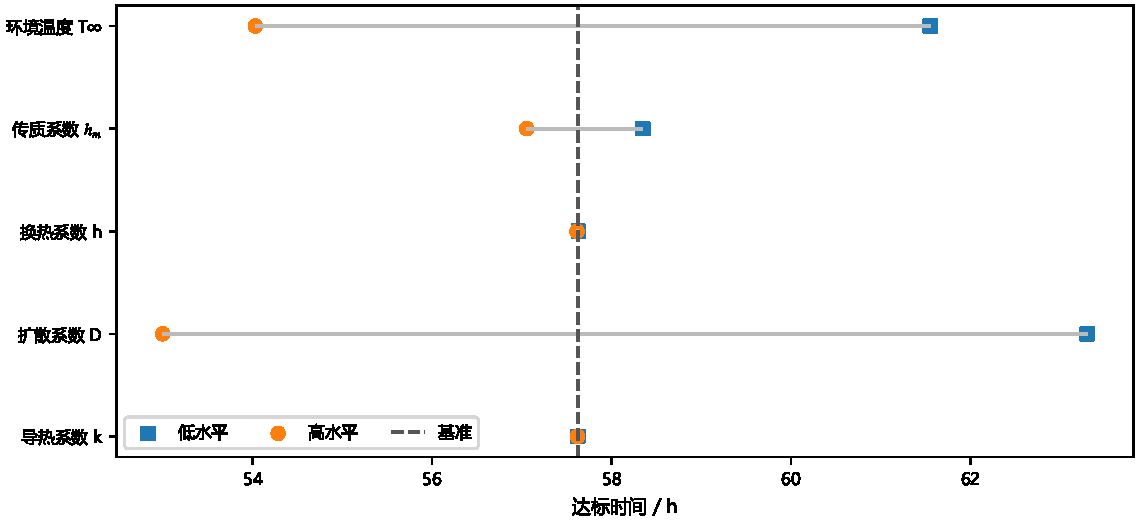
\includegraphics[width=0.82\linewidth]{analysis/fig9_sensitivity.pdf}
  \caption{参数扰动对达标时间的影响；$h_m$表示传质系数}
\end{figure}
\begin{figure}[htbp]
  \centering
  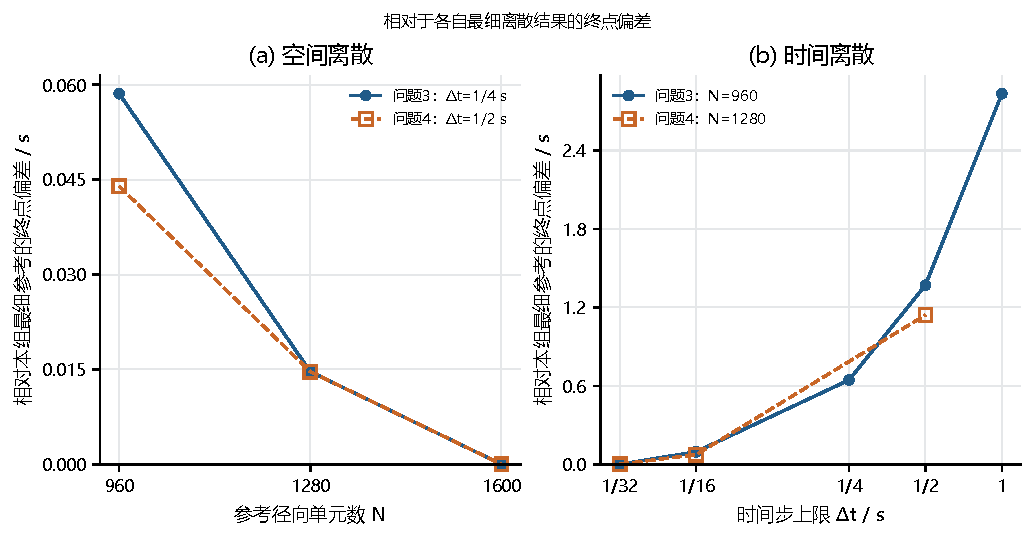
\includegraphics[width=0.82\linewidth]{q4/figures/fig8_combined_convergence.pdf}
  \caption{问题三、四空间和时间加密的终点收敛}
\end{figure}


% ==================== 可复制的排版骨架（默认禁用） ====================
% 图片/流程图：图片置于 figures 文件夹。填写标题后再使用。
% \begin{figure}[htbp]
%   \centering
%   \includegraphics[width=0.8\linewidth]{figures/filename.pdf}
%   \caption{} % 填写实际图名。
%   \label{fig:key}
% \end{figure}
% 图的交叉引用：图~\ref{fig:key}。
%
% 公式：填写实际数学表达式后再启用。
% \begin{equation}
%   % 在此填写公式。
%   \label{eq:key}
% \end{equation}
% 公式的交叉引用：式~\eqref{eq:key}。
%
% 带编号三线表：填入真实表名和数据后再启用。
% \begin{table}[htbp]
%   \centering
%   \caption{} % 填写实际表名。
%   \label{tab:key}
%   \begin{tabular}{ccc}
%     \toprule
%      & & \\
%     \midrule
%      & & \\
%     \bottomrule
%   \end{tabular}
% \end{table}
% 表的交叉引用：表~\ref{tab:key}。
% 章节交叉引用：第~\ref{sec:problem1}~节。
% 新增骨架时请使用唯一标签，避免重复 label。

\end{document}
